
\begin{center}
	\centering
\begin{table}[ht]
	\begin{tabular}{cc}
		\begin{subfigure}{0.4\textwidth}\centering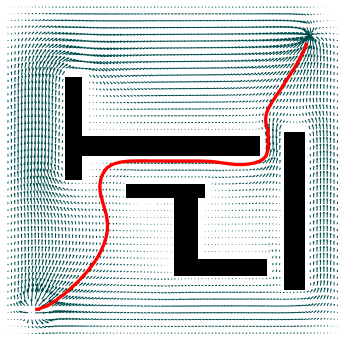
\includegraphics[width=0.9\linewidth]{figs/11/fig1}\caption{الخريطة الأولى}\label{11:fig:1}\end{subfigure}&
		\begin{subfigure}{0.4\textwidth}\centering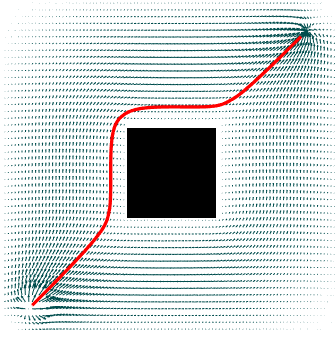
\includegraphics[width=0.9\linewidth]{figs/11/fig2}\caption{الخريطة الثانية}\label{11:fig:2}\end{subfigure}\\
		\newline
		\begin{subfigure}{0.4\textwidth}\centering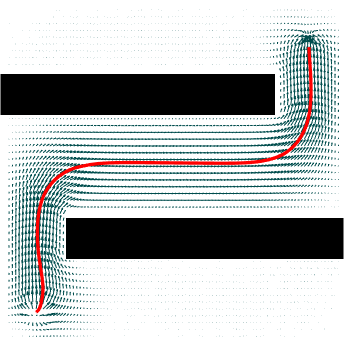
\includegraphics[width=0.9\linewidth]{figs/11/fig3}\caption{الخريطة الثالثة}\label{11:fig:3}\end{subfigure}&
		\begin{subfigure}{0.4\textwidth}\centering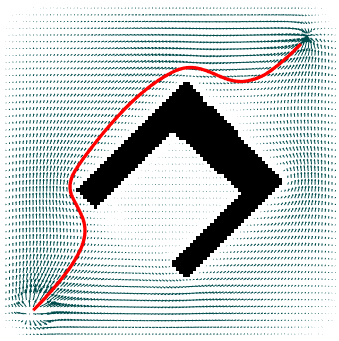
\includegraphics[width=0.9\linewidth]{figs/11/fig4}\caption{الخريطة الرابعة}\label{11:fig:4}\end{subfigure}\\
	\end{tabular}
	\caption{أداء الخوارزمية لعدة خرائط}
	\label{tab:mytable}
\end{table}
\end{center}
